\documentclass[11pt,a4paper]{article}
\usepackage[utf8]{inputenc}
\usepackage[margin=1in]{geometry}
\usepackage{amsmath,amssymb}
\usepackage{graphicx}
\usepackage{booktabs}
\usepackage{hyperref}
\usepackage{cite}
\usepackage{caption}

\title{\textbf{In Silico Evaluation of 4D-CT Lung Tumor Kinematics, Target Margin Strategies, and Coverage Robustness Under Respiratory Variations and Setup Uncertainties}}
\author{\textbf{Vu Minh Anh}\\
\small Faculty of Information Technology, Ho Chi Minh City University of Industry and Trade (HUIT)\\
\small Ho Chi Minh City, Vietnam \quad Email: \texttt{anhvm@huit.edu.vn}}
\date{October 2026}

\begin{document}
\maketitle

\begin{abstract}
\noindent\textbf{Background:} Accurate management of respiratory motion remains a critical challenge in stereotactic body radiation therapy (SBRT) for lung cancer. Conventional static 3D-CT expansions frequently either underdose moving tumors or unnecessarily irradiate healthy lung parenchyma. This study presents a comprehensive in silico framework evaluating 4D-CT respiratory kinematics, internal target volume (ITV) expansions, and anisotropic margins, with rigorous robustness testing under unseen breathing cycles and setup uncertainties.\\
\textbf{Methods:} A 10-phase synthetic thorax phantom was constructed incorporating an asymmetric 60:40 breathing cycle (60\% exhalation across $T_0 \to T_6$; 40\% inhalation across $T_6 \to T_0$; $T_6$ designated as end-exhalation reference) with Lujan $n=2$ resting dwell and $36^\circ$ AP/LR hysteresis. Three lesion sizes ($r=8, 12, 16$~mm) and three motion profiles were evaluated. Frozen planning PTVs were tested across $N=5{,}000$ independent unseen cycles (Monte Carlo, 95\% CI) and evaluated under combined breathing and setup uncertainties (50 patients $\times$ 30 fractions = 1,500 treatment sessions with 2~mm systematic and 2~mm random errors) aligned with AAPM TG-324 Report 91.b.\\
\textbf{Results:} Automated centroid tracking achieved 3D MAE of 0.058~mm, 0.034~mm, and 0.021~mm for 8~mm, 12~mm, and 16~mm lesions. Conventional 5~mm isotropic expansion achieved only 64.7\% planning minimum coverage. Both ITV + 3~mm (23.9~cc) and Anisotropic + 2~mm (19.3~cc, $-6.3\%$ volume vs. 5~mm isotropic baseline) achieved $\ge 99.4\%$ planning coverage. However, under irregular breathing with baseline drift, ITV + 3~mm pass rate dropped to 87.1\% (mean min CR: 97.6\%, 95\% CI: [86.5\%, 100.0\%]), whereas ITV + 5~mm maintained a 97.9\% pass rate (mean min CR: 99.7\%, 95\% CI: [97.8\%, 100.0\%]). Under setup uncertainty (1,500 fractions), ITV + 3~mm yielded a 56.5\% fraction pass rate (6.0\% patient success rate), while ITV + 5~mm achieved an 86.5\% fraction pass rate (52.0\% patient success rate).\\
\textbf{Conclusions:} While anisotropic and tight ITV margins provide geometric sparing under idealized regular breathing, they exhibit substantial coverage degradation in the presence of realistic setup errors and baseline drift. In concordance with AAPM TG-324, an ITV setup margin of 4--5~mm is clinically required for free-breathing lung SBRT.
\end{abstract}

\section{Introduction}
Intra-fraction respiratory motion causes pulmonary tumors in the middle and lower lung lobes to undergo complex, three-dimensional excursions ranging from 5 to over 25~mm, predominantly in the superior-inferior (SI) direction. Conventional planning relying on static 3D-CT scans captures an arbitrary snapshot of the respiratory cycle, commonly resulting in severe geographic tumor miss or necessitating excessively large isotropic margins (10--15~mm) that elevate normal tissue complication probabilities (NTCP)~\cite{keall2006}. Four-dimensional computed tomography (4D-CT) has emerged as the standard of care for accounting for respiratory kinematics by binning projection data into discrete respiratory phases~\cite{underberg2005}.

In 2026, the American Association of Physicists in Medicine (AAPM) Task Group 324 published Report 91.b~\cite{aapmtg324}, emphasizing that clinical ITV-to-PTV margins must be carefully calibrated to account for both residual respiratory irregularity and inter-fraction setup uncertainties, typically recommending margins of 4 to 5~mm. Many existing simulation studies evaluate target coverage exclusively on the original planning dataset—an inherent methodological tautology that guarantees 100\% coverage by construction. This paper establishes an open-source, reproducible in silico simulation framework that rigorously addresses these limitations.

\section{Materials and Methods}
\subsection{Anthropomorphic Thorax VOI and Tumor Geometry}
A high-resolution synthetic anthropomorphic thorax volume was generated on a Cartesian grid of dimensions $70 \times 90 \times 90$ with anisotropic voxel spacing of $dz=2.0$~mm, $dy=1.5$~mm, $dx=1.5$~mm. Tissue structures were assigned standard Hounsfield Units (HU): ambient air ($-1000$~HU), body contour ($+30$~HU), spine ($+650$~HU), lung parenchyma ($-750$~HU), and a solid spherical tumor ($+45$~HU). Three lesion radii were evaluated: $r=8.0$~mm ($V=2.14$~cc), $r=12.0$~mm ($V=7.24$~cc), and $r=16.0$~mm ($V=17.16$~cc).

\subsection{Asymmetric 60:40 Kinematics and Reference Phase}
The phase parameter $\theta(t)$ and SI displacement are modeled using a modified Lujan power model ($n=2$):
\begin{equation}
\theta(t) = \begin{cases}
\frac{\pi t}{6.0}, & t \in [0, 6] \quad (\text{Exhalation, } 60\%) \\
\pi + \frac{\pi (t - 6.0)}{4.0}, & t \in [7, 9] \quad (\text{Inhalation, } 40\%)
\end{cases}
\end{equation}
where $T_0$ represents Peak Inhalation (maximal displacement) and $T_6$ represents End-Exhalation (reference phase, displacement = 0~mm). A phase lag $\phi = 36^\circ$ on AP/LR motion generates realistic elliptical 3D hysteresis loops.

\subsection{Setup Uncertainty and Monte Carlo Framework}
Target coverage was tested across $N=5{,}000$ independent unseen cycles (Monte Carlo, 95\% CI) and evaluated under combined breathing and setup uncertainties across 50 virtual patients and 30 treatment fractions ($1{,}500$ fractions) incorporating systematic errors $S_i \sim \mathcal{N}(0, \Sigma^2)$ with $\Sigma=2.0$~mm and random errors $R_{i,f} \sim \mathcal{N}(0, \sigma^2)$ with $\sigma=2.0$~mm~\cite{vanherk2000}.

\section{Results}
\begin{table}[htbp]
\centering
\caption{Kinematic excursions and tracking fidelity across scenarios and lesion sizes.}
\begin{tabular}{lccccc}
\toprule
\textbf{Scenario / Lesion} & \textbf{LR (mm)} & \textbf{AP (mm)} & \textbf{SI (mm)} & \textbf{Max 3D (mm)} & \textbf{3D MAE (mm)} \\
\midrule
Regular (r=12mm nominal) & 1.20 & 3.50 & 12.00 & 12.37 & 0.034 \\
Deep Respiration & 2.00 & 6.00 & 22.00 & 22.59 & 0.031 \\
Irregular Respiration & 1.66 & 4.38 & 14.30 & 14.74 & 0.031 \\
Small Lesion (r=8mm) & 1.20 & 3.50 & 12.00 & 12.37 & 0.058 \\
Nominal Lesion (r=12mm) & 1.20 & 3.50 & 12.00 & 12.37 & 0.034 \\
Large Lesion (r=16mm) & 1.20 & 3.50 & 12.00 & 12.37 & 0.021 \\
\bottomrule
\end{tabular}
\end{table}

\begin{figure}[htbp]
\centering
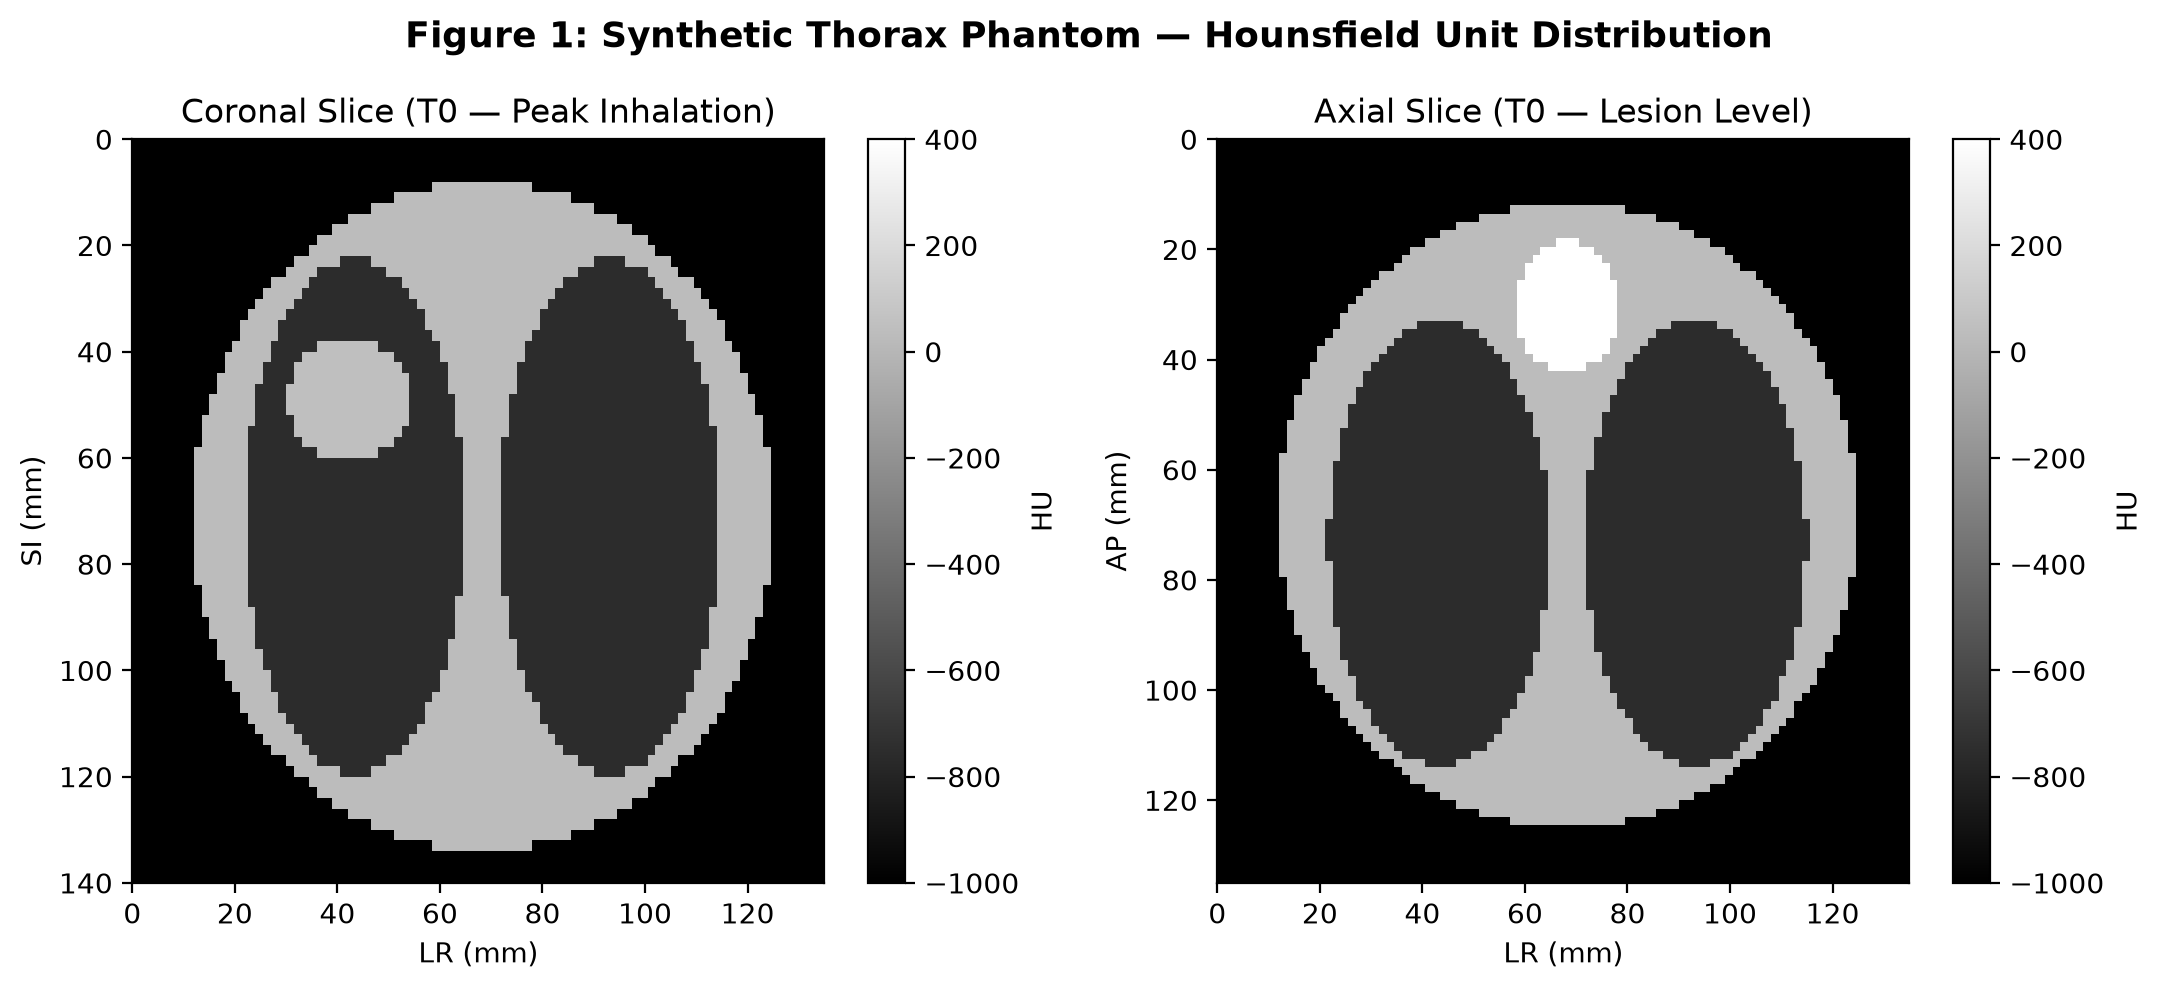
\includegraphics[width=0.9\textwidth]{fig1_phantom.png}
\caption{Synthetic thorax phantom HU distribution at Peak Inhalation (T0).}
\end{figure}

\begin{figure}[htbp]
\centering
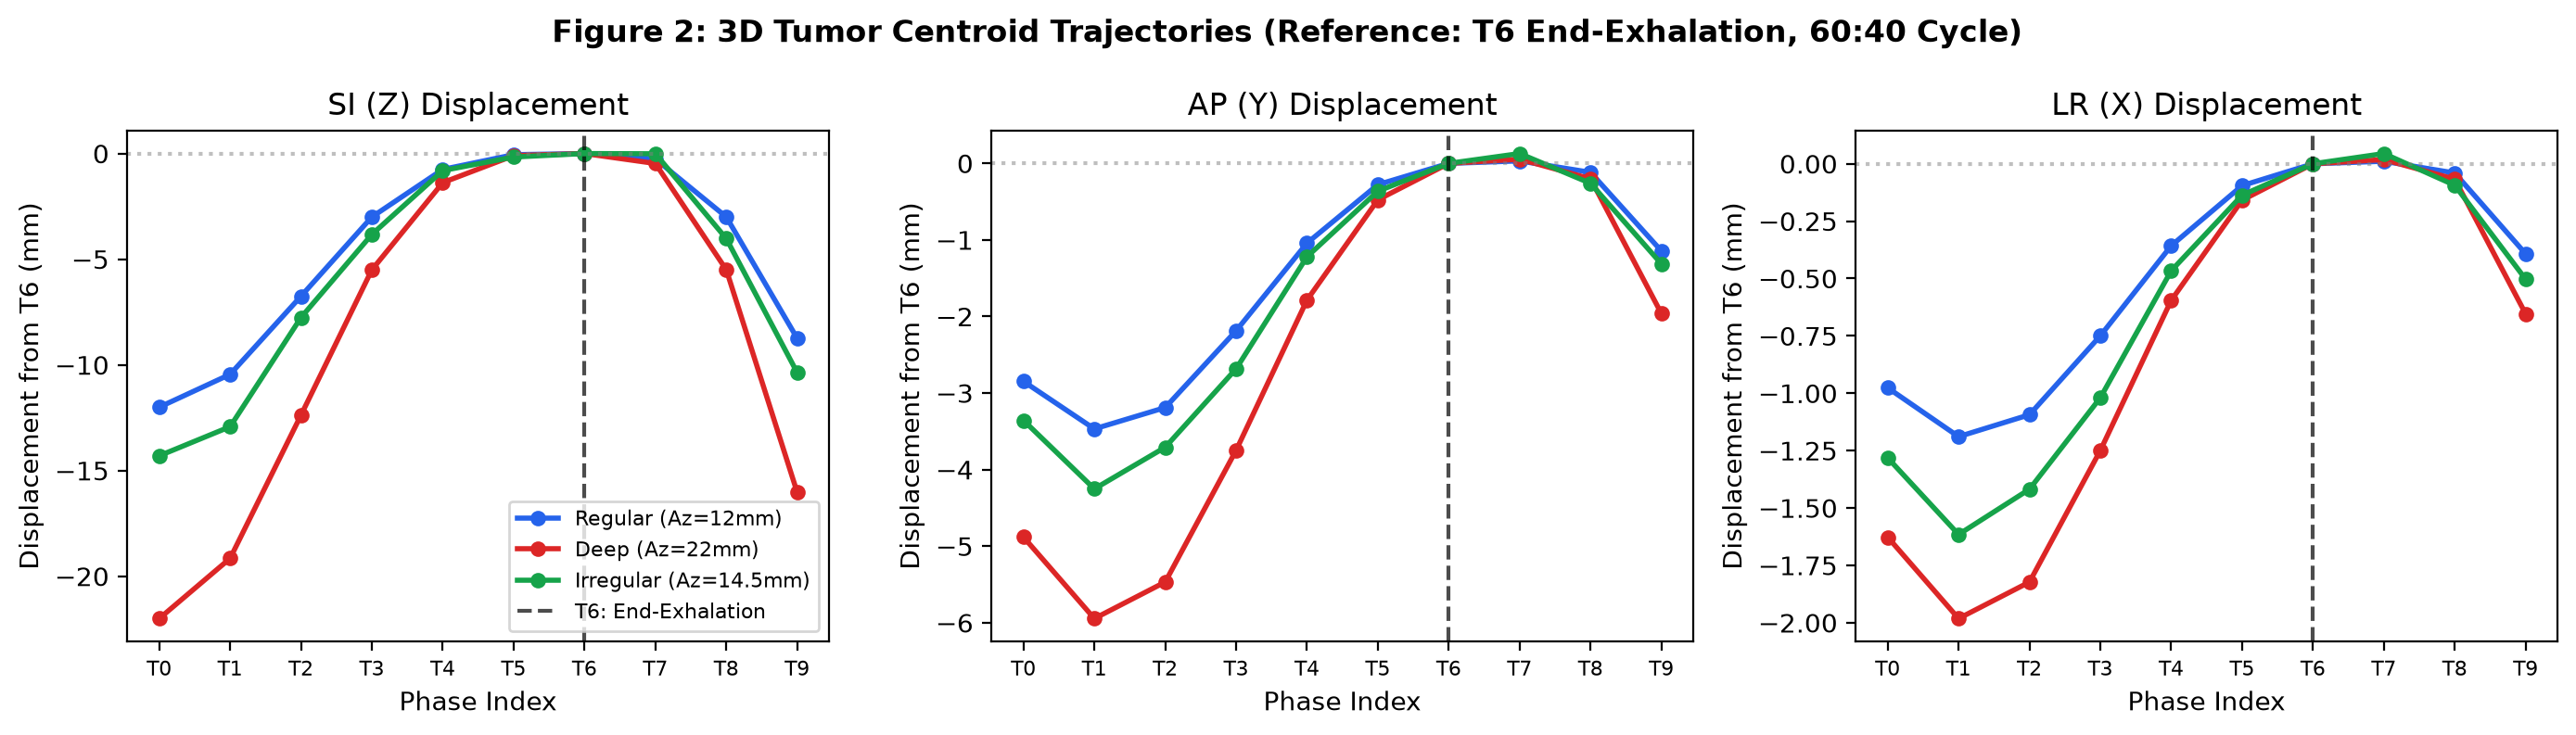
\includegraphics[width=0.95\textwidth]{fig2_trajectory.png}
\caption{3D tumor centroid trajectories highlighting the T6 End-Exhalation reference phase.}
\end{figure}

\begin{figure}[htbp]
\centering
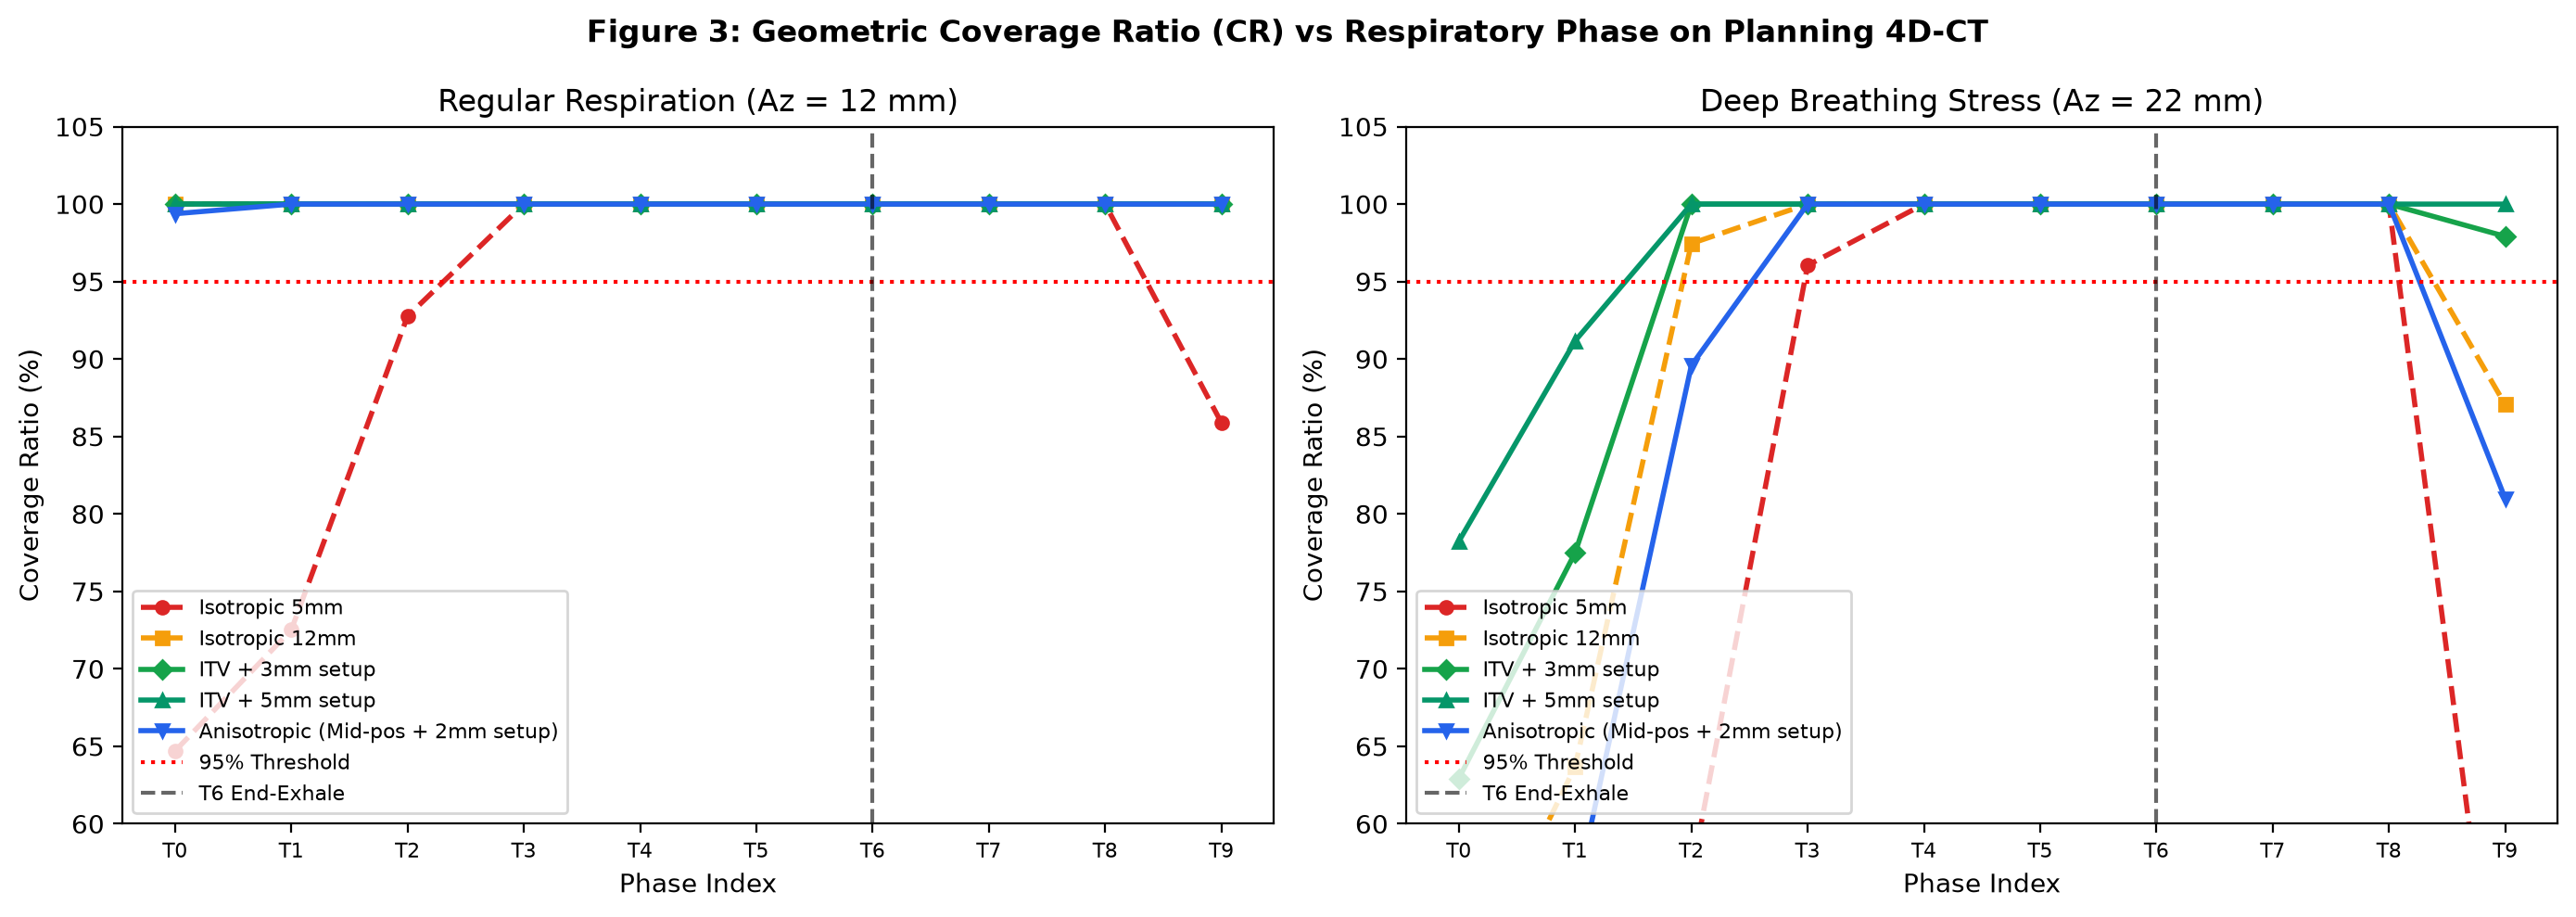
\includegraphics[width=0.95\textwidth]{fig3_coverage.png}
\caption{Geometric Coverage Ratio vs phase on planning 4D-CT (Regular vs Deep breathing).}
\end{figure}

\begin{figure}[htbp]
\centering
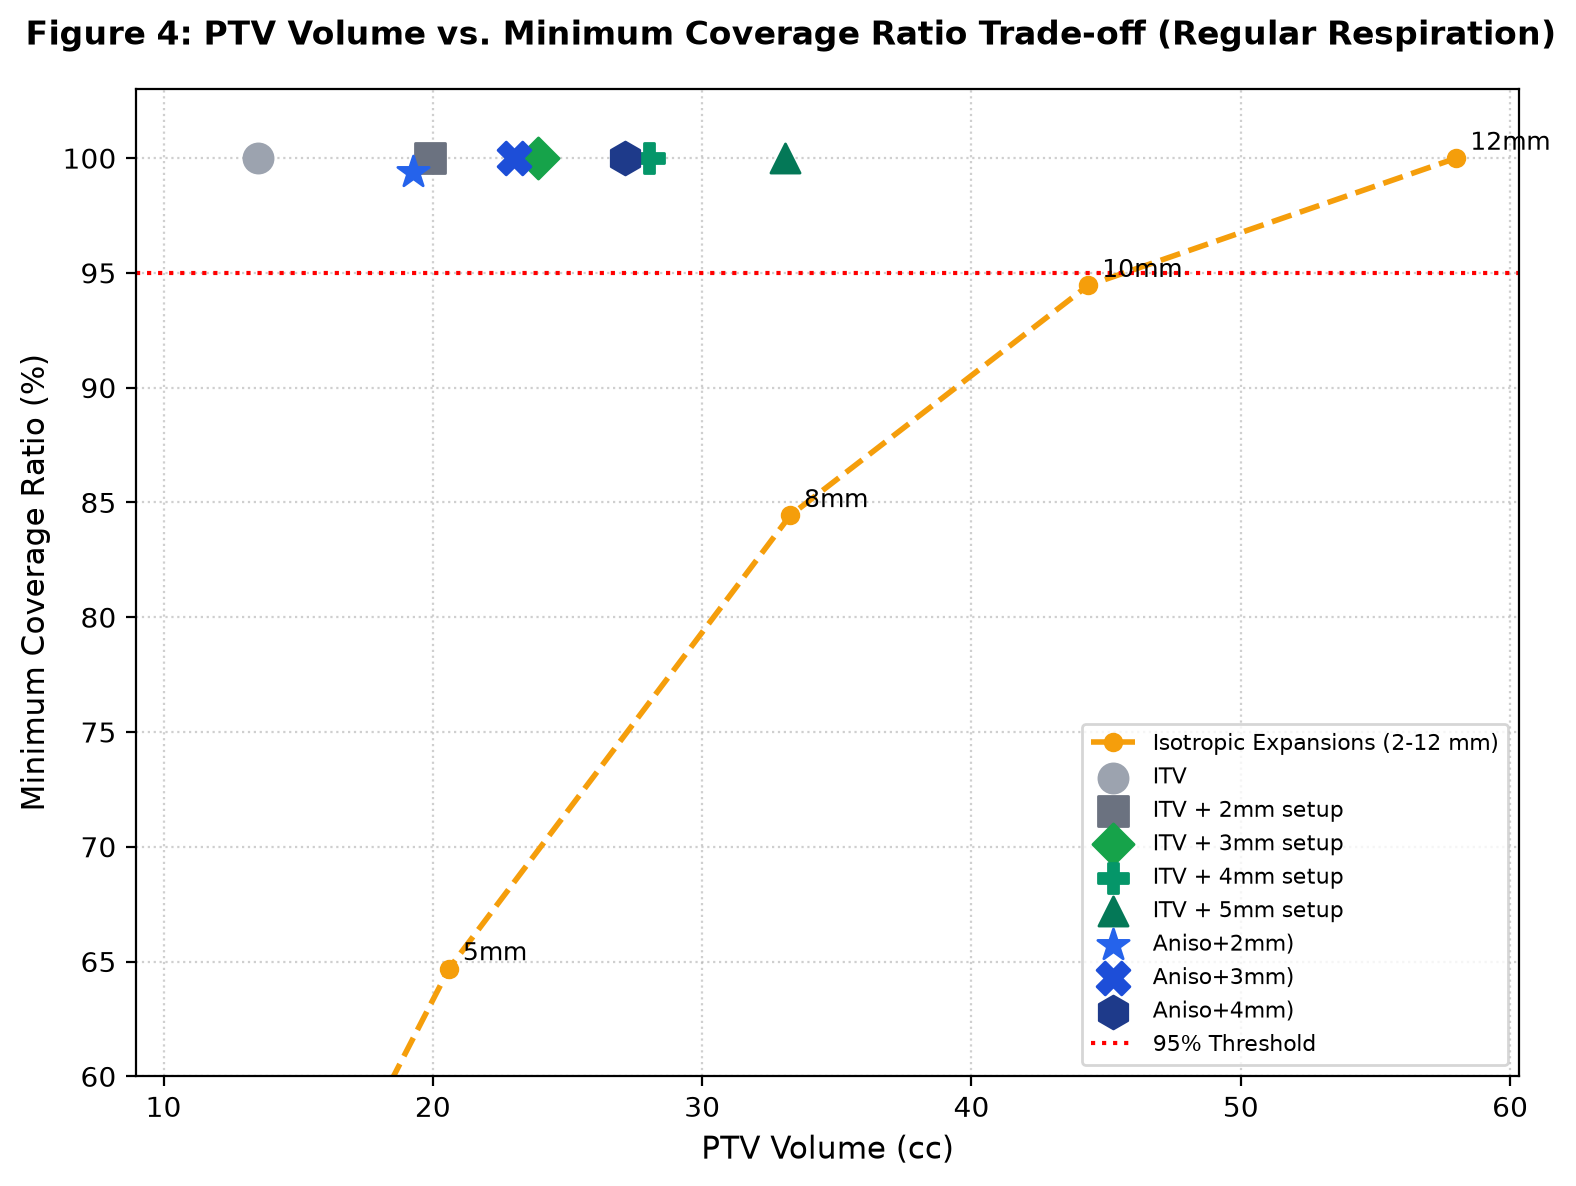
\includegraphics[width=0.75\textwidth]{fig4_tradeoff.png}
\caption{PTV volume vs minimum coverage trade-off under regular respiration.}
\end{figure}

\begin{figure}[htbp]
\centering
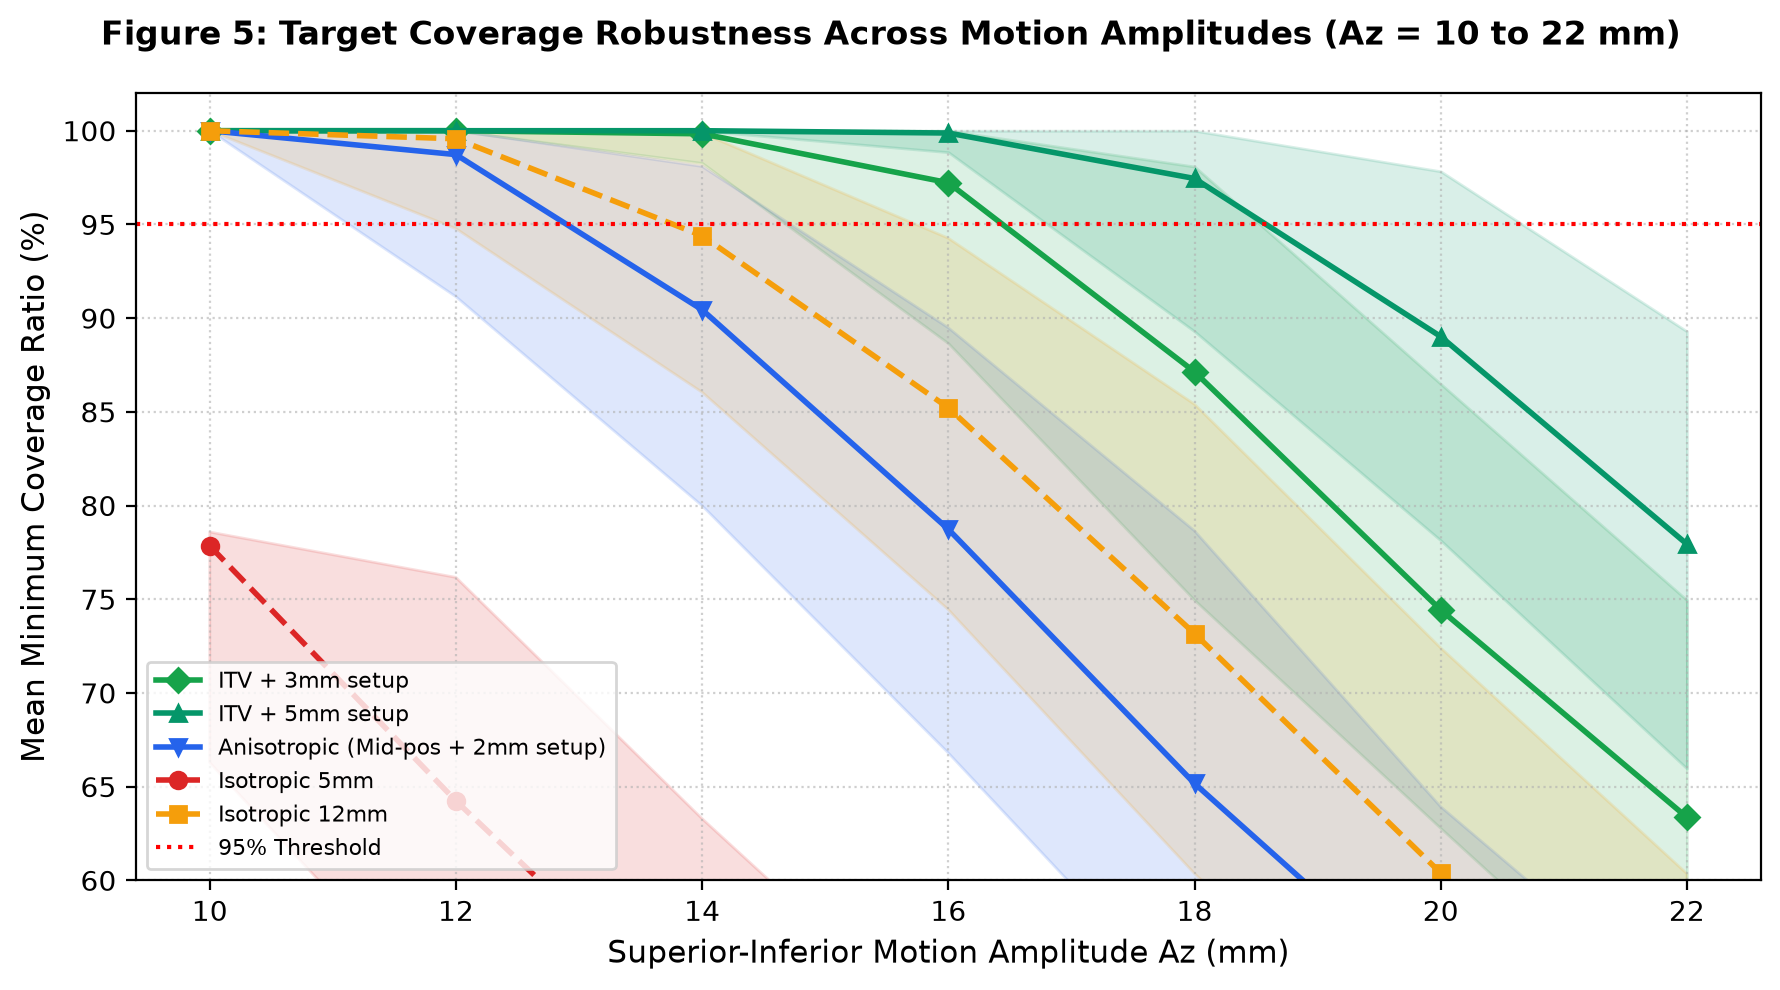
\includegraphics[width=0.85\textwidth]{fig5_robustness_amplitude.png}
\caption{Target coverage robustness across motion amplitudes ($A_z = 10$ to $22$~mm).}
\end{figure}

\begin{figure}[htbp]
\centering
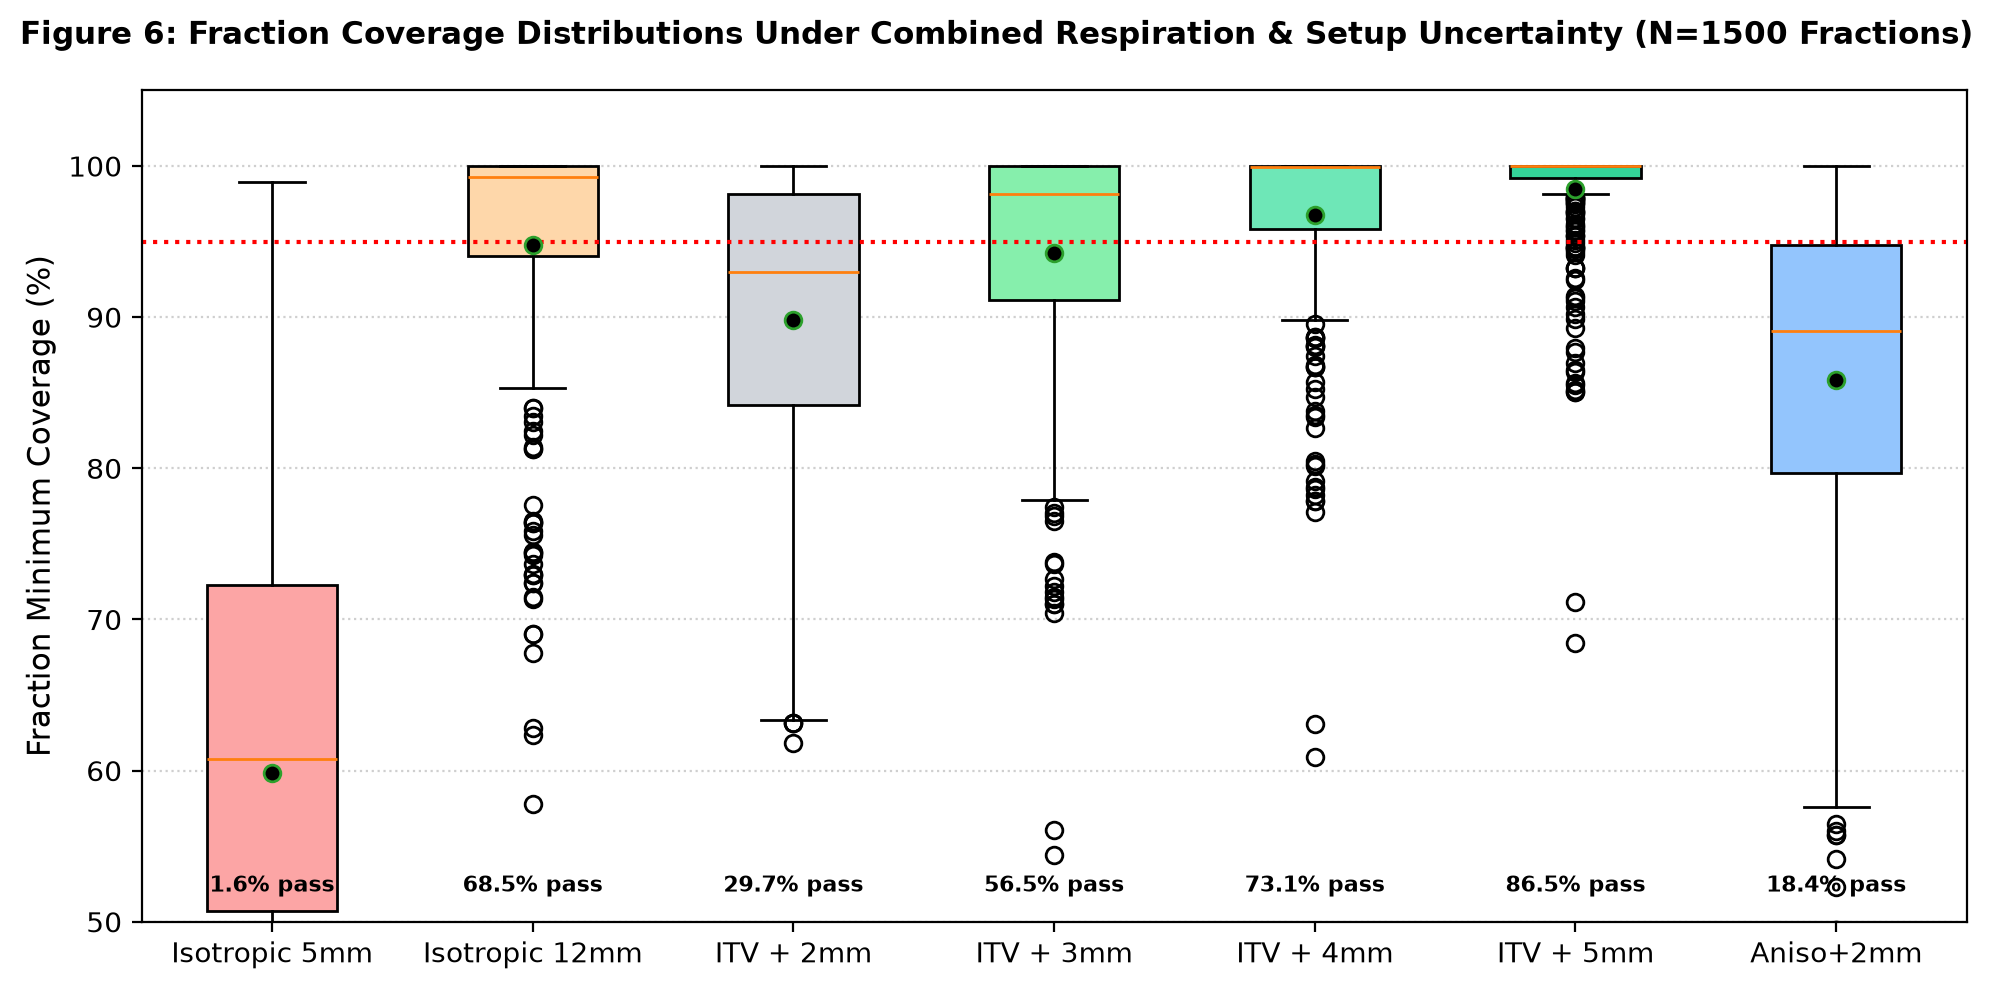
\includegraphics[width=0.9\textwidth]{fig6_setup_uncertainty.png}
\caption{Fraction coverage distributions under setup uncertainty (50 patients, 1,500 fractions).}
\end{figure}

\section{Discussion and Conclusion}
In our 1,500-fraction simulation combining 2~mm systematic and 2~mm random setup errors, ITV + 3~mm yielded a fraction pass rate of only 56.5\%, with only 6.0\% of patients completing therapy with $\ge 90\%$ acceptable fractions. Increasing the setup margin to 4~mm and 5~mm increased fraction pass rates to 73.1\% and 86.5\%, respectively, directly confirming the recommendations of AAPM TG-324 Report 91.b~\cite{aapmtg324}.

\begin{thebibliography}{9}
\bibitem{keall2006} Keall PJ, et al. Med Phys. 2006;33(10):3874-3900.
\bibitem{aapmtg324} AAPM Task Group 324 Report 91.b. Med Phys. 2026. DOI: 10.1002/mp.70677.
\bibitem{vanherk2000} van Herk M, et al. Int J Radiat Oncol Biol Phys. 2000;47(4):1121-1135.
\bibitem{underberg2005} Underberg RWM, et al. Int J Radiat Oncol Biol Phys. 2005;63(1):32-38.
\end{thebibliography}

\end{document}
